% You should title the file with a .tex extension (hw1.tex, for example)
\documentclass[a4paper, 11pt]{article}

\usepackage{amsmath}
\usepackage{amssymb}
\usepackage{fancyhdr}
\usepackage{graphicx}

\usepackage[margin=1in]{geometry}

\newcommand{\question}[2] {\vspace{.25in} \hrule\vspace{0.5em}
\noindent{\bf #1: #2} \vspace{0.5em}
\hrule \vspace{.10in}}
\renewcommand{\part}[1] {\vspace{.10in} {\bf (#1)}}

\newcommand{\myname}{Natthakan Euaumpon}
\newcommand{\myemail}{natthakaneuaumpon@gmail.com}
\newcommand{\myhwnum}{1}

\setlength{\parindent}{0pt}
\setlength{\parskip}{5pt plus 1pt}
 
\pagestyle{fancyplain}
\lhead{\fancyplain{}{\textbf{HW\myhwnum}}}      % Note the different brackets!
\rhead{\fancyplain{}{\myname\\ \myemail}}
\chead{\fancyplain{}{ICCS310 }}

\begin{document}

\medskip                        % Skip a "medium" amount of space
                                % (latex determines what medium is)
                                % Also try: \bigskip, \littleskip

\thispagestyle{plain}
\begin{center}                  % Center the following lines
{\Large ICCS310: Exam \myhwnum} \\
\myname \\
\myemail \\
February 2021 \\
\end{center}

\question{2}{}
We get that: $L^+ = LL^*$\\
So, $L^{++} = LL^*(LL^*)^*$\\
Therefore $L^{++R} = (LL^*(LL^*)^*)^R$\\
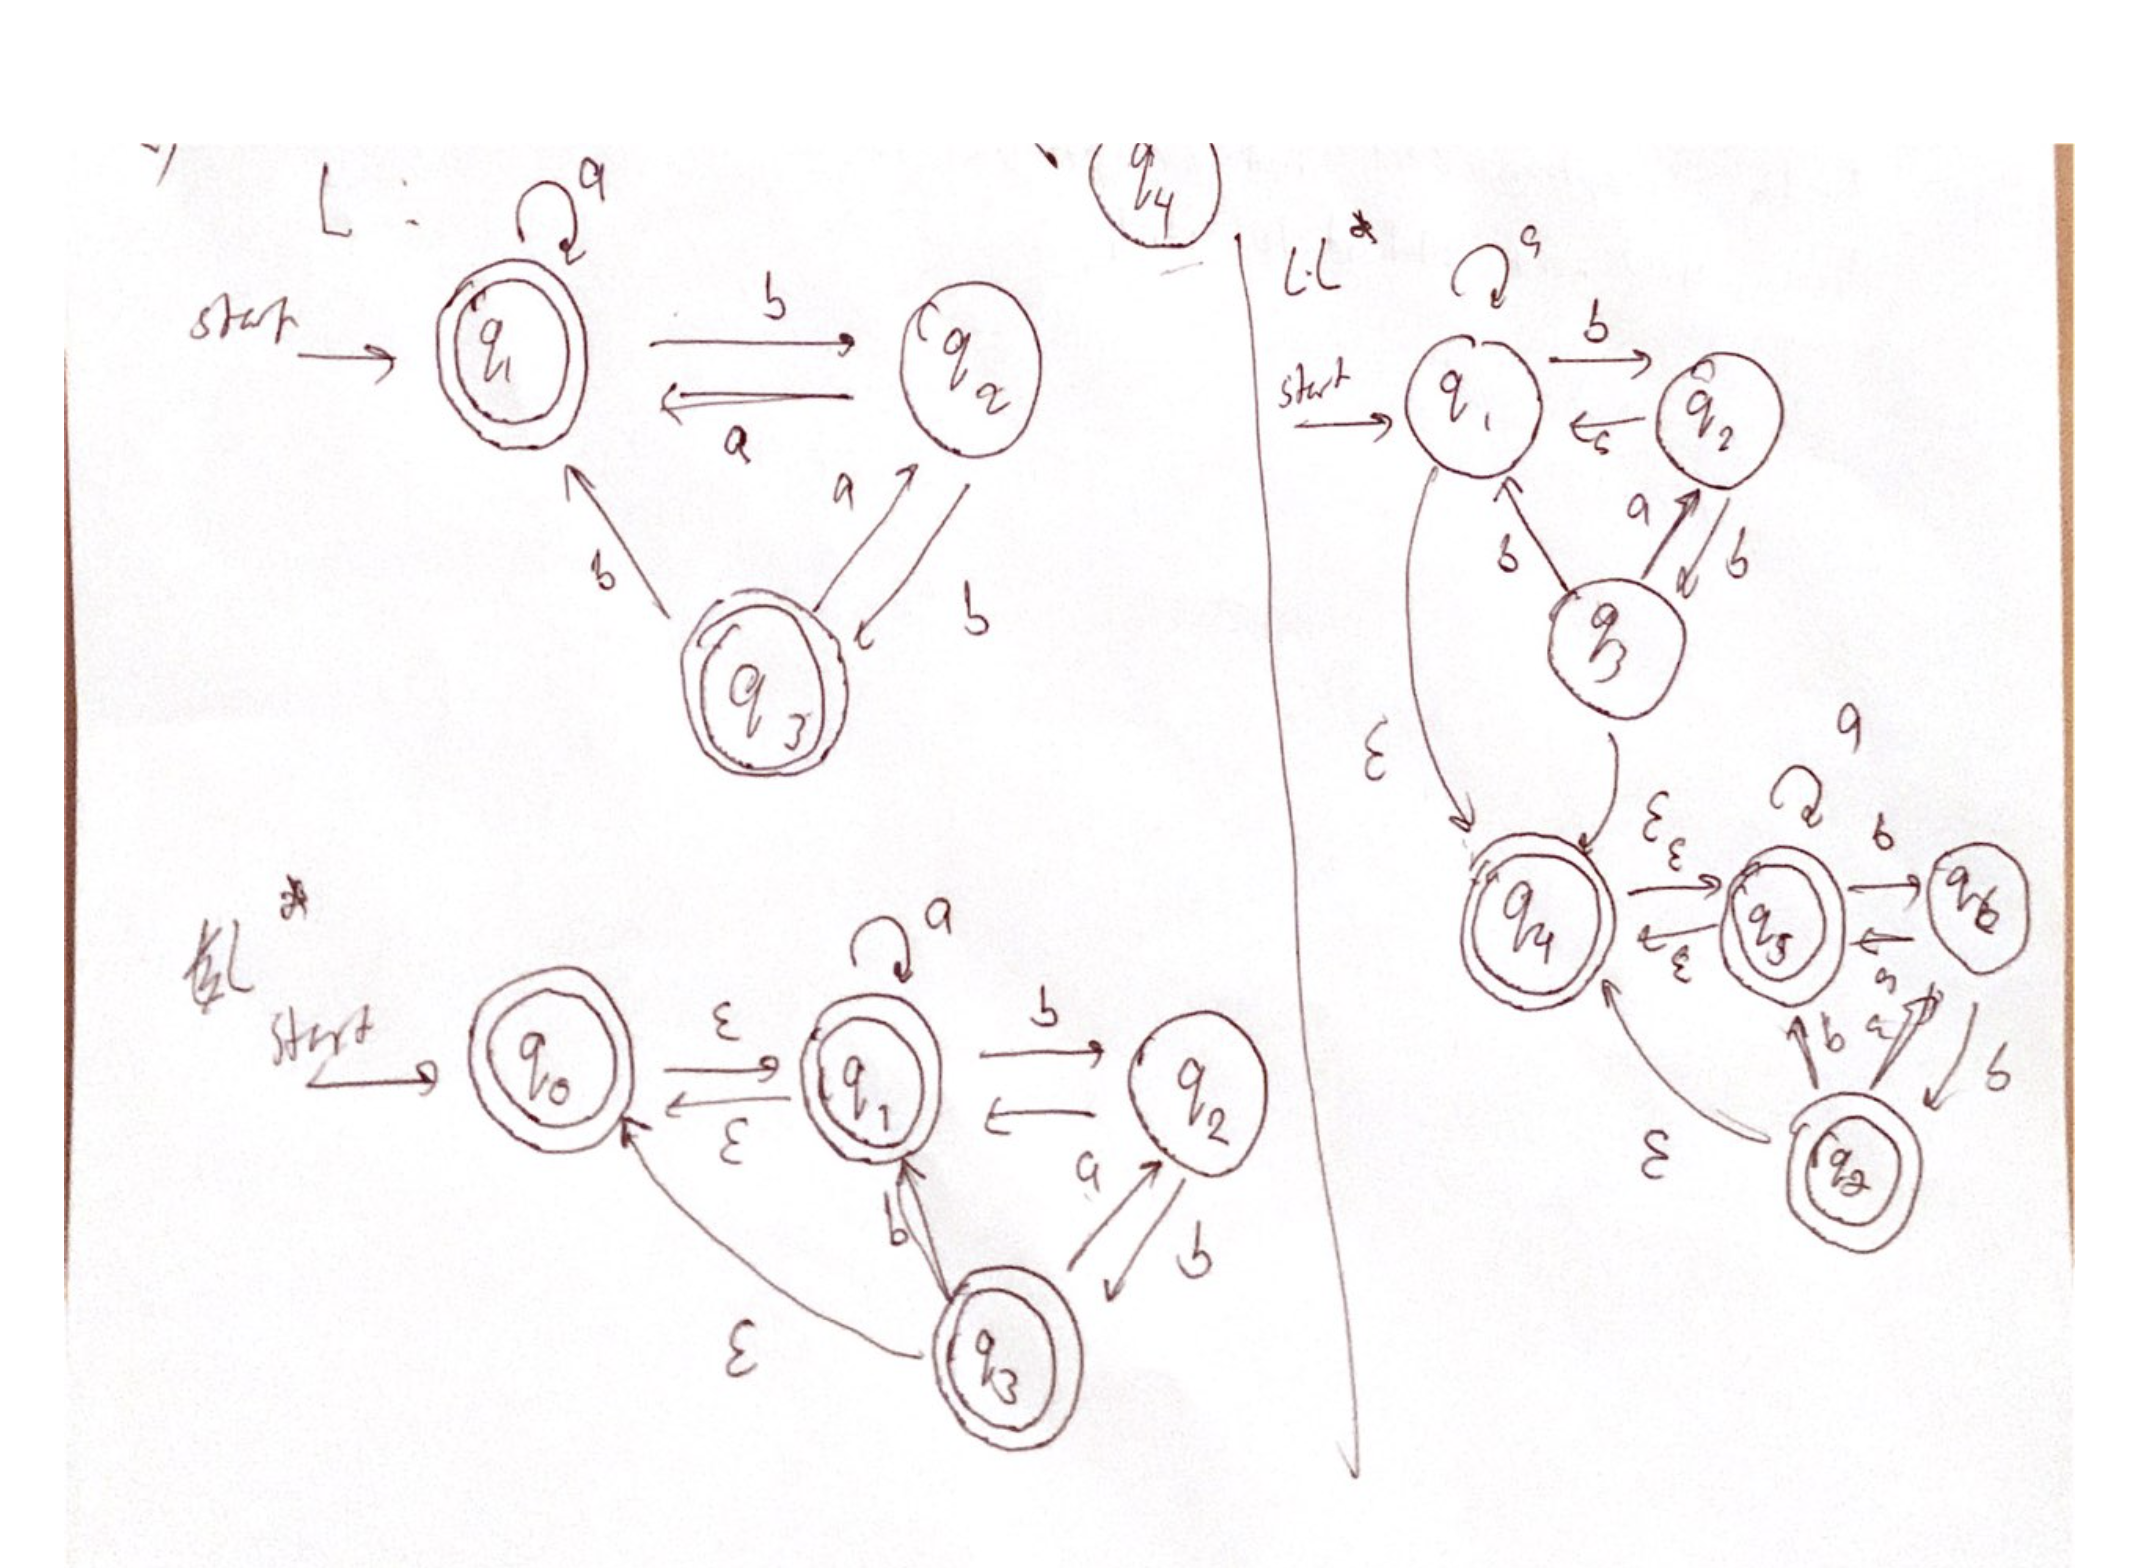
\includegraphics[width=\textwidth]{Q2-1.png}\\
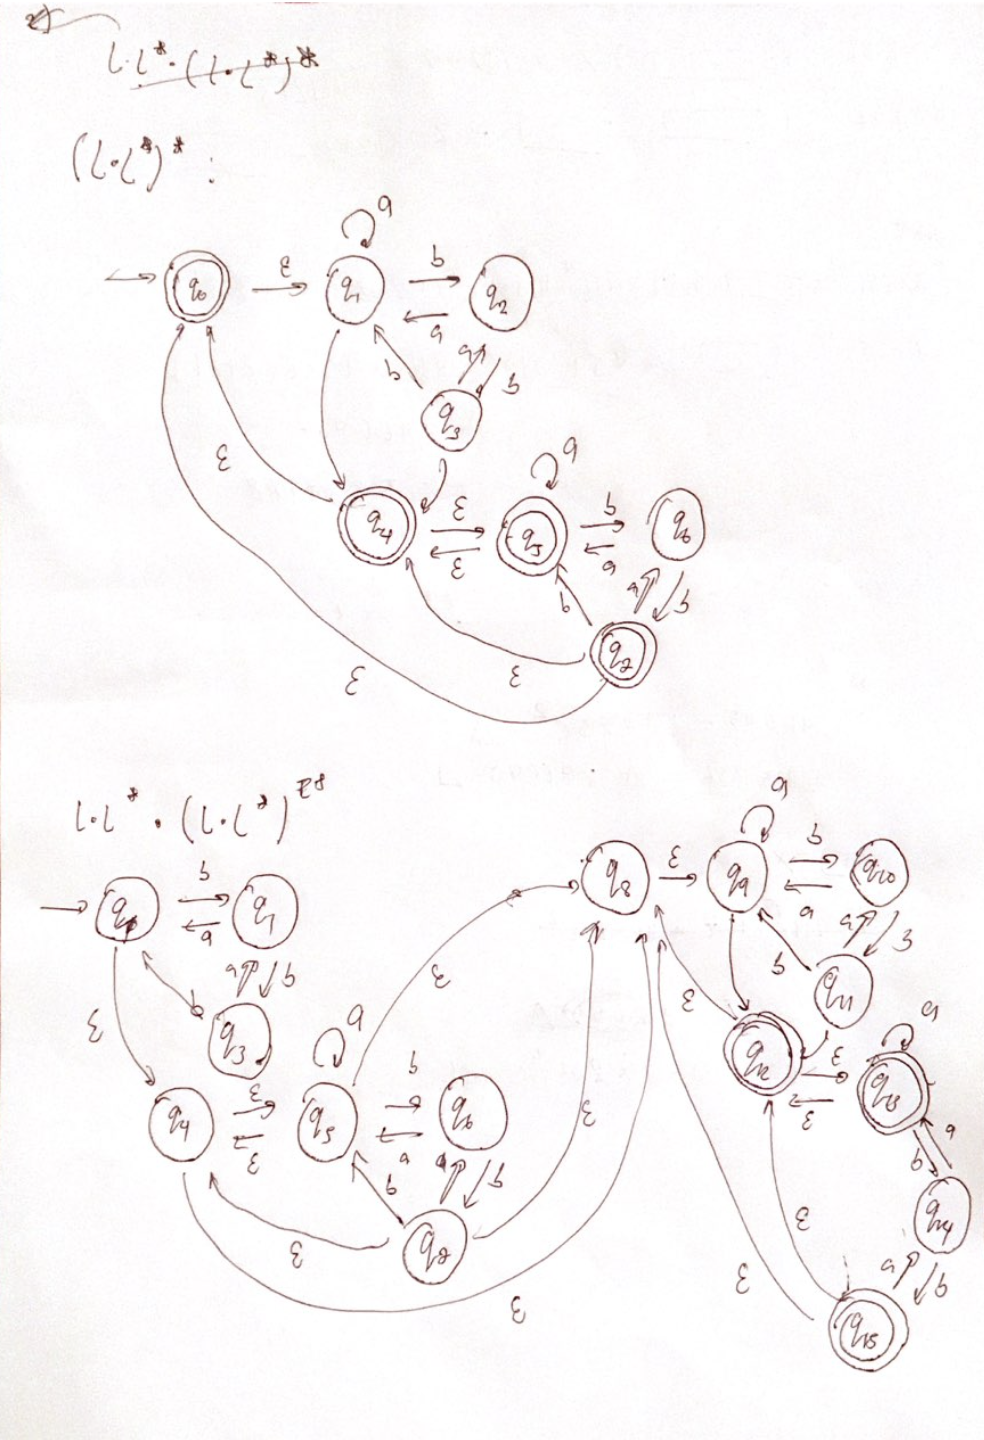
\includegraphics[width=\textwidth]{Q2-2.png}\\
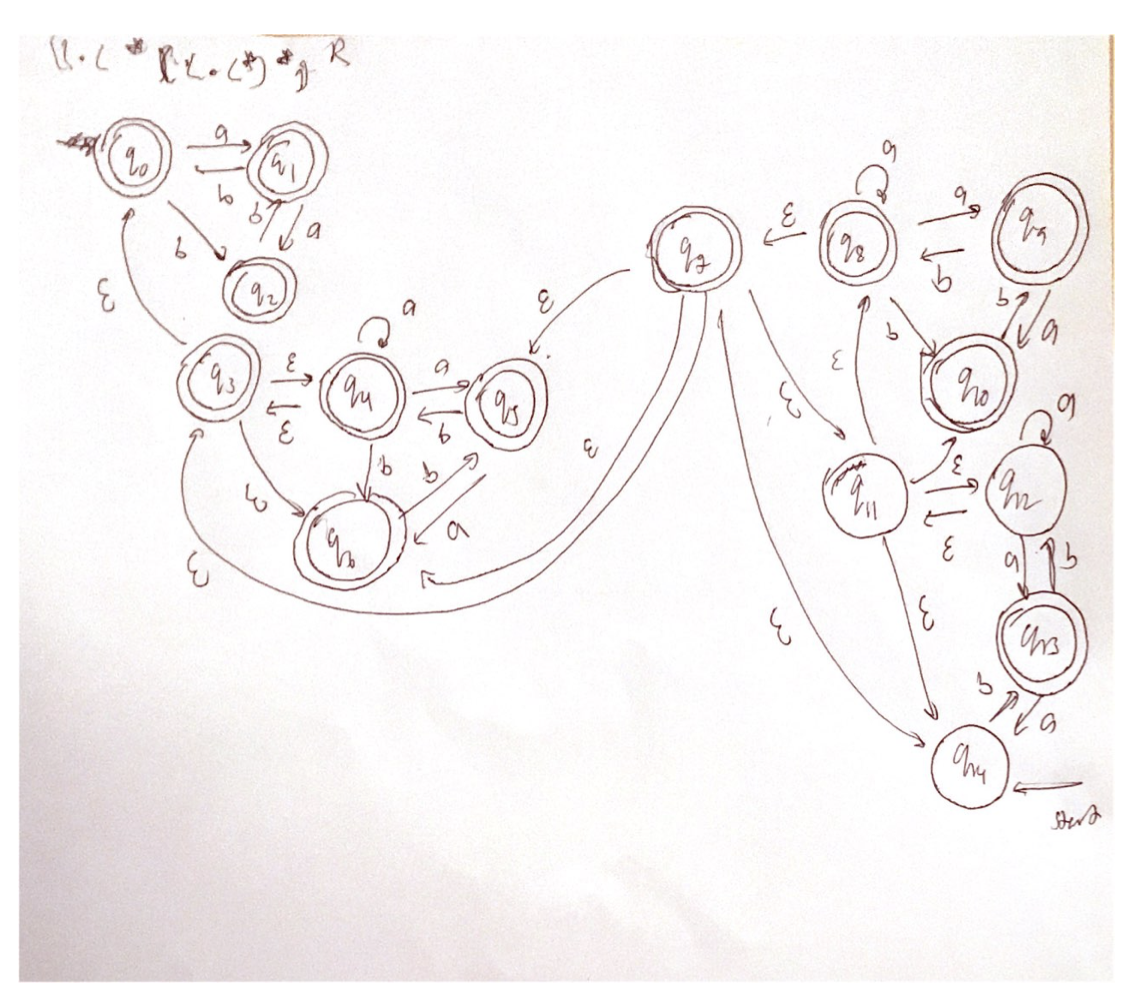
\includegraphics[width=\textwidth]{Q2-3.png}

\question{4}{After add toc part}
During the first half of the exam already add value string toc to hash value.\\
We get the hash value of 246045.\\
So we have $h(y) = (246045-x[0] \cdot 256^30 - x[1] \cdot 256^29) \mod 7513199$

\end{document}

